\documentclass[12pt,a4paper]{article}
\usepackage[utf8]{inputenc}
\usepackage{amsmath}
\usepackage{amsfonts}
\usepackage{amssymb}
\usepackage[brazil]{babel}
\usepackage{indentfirst}
\usepackage{url}
\usepackage{listings}
\usepackage{color}
\RequirePackage{graphicx}


%%%%%%%%%%Codigos para o HTML%%%%%%%%%%%%%%%%%%%%%%%%%%%%%%%%

\definecolor{editorGray}{rgb}{0.95, 0.95, 0.95}
\definecolor{editorOcher}{rgb}{1, 0.5, 0} % #FF7F00 -> rgb(239, 169, 0)
\definecolor{editorGreen}{rgb}{0, 0.5, 0} % #007C00 -> rgb(0, 124, 0)
\usepackage{upquote}
\usepackage{listings}
\lstdefinelanguage{JavaScript}{
  morekeywords={typeof, new, true, false, catch, function, return, null, catch, switch, var, if, in, while, do, else, case, break},
  morecomment=[s]{/*}{*/},
  morecomment=[l]//,
  morestring=[b]",
  morestring=[b]'
}

\lstdefinelanguage{HTML5}{
        language=html,
        sensitive=true, 
        alsoletter={<>=-},
        otherkeywords={
        % HTML tags
        <html>, <head>, <title>, </title>, <meta, />, </head>, <body>,
        <canvas, \/canvas>, <script>, </script>, </body>, </html>, <!, html>, <style>, </style>, ><
        },  
        ndkeywords={
        % General
        =,
        % HTML attributes
        charset=, id=, width=, height=,
        % CSS properties
        border:, transform:, -moz-transform:, transition-duration:, transition-property:, transition-timing-function:
        },  
        morecomment=[s]{<!--}{-->},
        tag=[s]
}

\lstset{%
    % Basic design
    backgroundcolor=\color{editorGray},
    basicstyle={\small\ttfamily},   
    frame=l,
    % Line numbers
    xleftmargin={0.75cm},
    numbers=left,
    stepnumber=1,
    firstnumber=1,
    numberfirstline=true,
    % Code design   
    keywordstyle=\color{blue}\bfseries,
    commentstyle=\color{darkgray}\ttfamily,
    ndkeywordstyle=\color{editorGreen}\bfseries,
    stringstyle=\color{editorOcher},
    % Code
    language=HTML5,
    alsolanguage=JavaScript,
    alsodigit={.:;},
    tabsize=2,
    showtabs=false,
    showspaces=false,
    showstringspaces=false,
    extendedchars=true,
    breaklines=true,        
    % Support for German umlauts
    literate=%
    {Ö}{{\"O}}1
    {Ä}{{\"A}}1
    {Ü}{{\"U}}1
    {ß}{{\ss}}1
    {ü}{{\"u}}1
    {ä}{{\"a}}1
    {ö}{{\"o}}1
}
%%%%%%%%%%%%%%%%%%%%%%%%%%%%%%%%Fim codigo HTML%%%%%%%%%%%%%%


%%%%%%%%%%%Codigo geral%%%%%%%%%%%%%%%%%%%%%%%%%%%%%%%%%%%%%%
\definecolor{mygreen}{rgb}{0,0.6,0}
\definecolor{mygray}{rgb}{0.5,0.5,0.5}
\definecolor{mymauve}{rgb}{0.58,0,0.82}

\lstset{ %
  backgroundcolor=\color{white},   % choose the background color; you must add \usepackage{color} or \usepackage{xcolor}; should come as last argument
  basicstyle=\footnotesize,        % the size of the fonts that are used for the code
  breakatwhitespace=false,         % sets if automatic breaks should only happen at whitespace
  breaklines=true,                 % sets automatic line breaking
  captionpos=b,                    % sets the caption-position to bottom
  commentstyle=\color{mygreen},    % comment style
  deletekeywords={...},            % if you want to delete keywords from the given language
  escapeinside={\%*}{*)},          % if you want to add LaTeX within your code
  extendedchars=true,              % lets you use non-ASCII characters; for 8-bits encodings only, does not work with UTF-8
  frame=single,	                   % adds a frame around the code
  keepspaces=true,                 % keeps spaces in text, useful for keeping indentation of code (possibly needs columns=flexible)
  keywordstyle=\color{blue},       % keyword style
  language=Octave,                 % the language of the code
  morekeywords={*,...},            % if you want to add more keywords to the set
  numbers=left,                    % where to put the line-numbers; possible values are (none, left, right)
  numbersep=5pt,                   % how far the line-numbers are from the code
  numberstyle=\tiny\color{mygray}, % the style that is used for the line-numbers
  rulecolor=\color{black},         % if not set, the frame-color may be changed on line-breaks within not-black text (e.g. comments (green here))
  showspaces=false,                % show spaces everywhere adding particular underscores; it overrides 'showstringspaces'
  showstringspaces=false,          % underline spaces within strings only
  showtabs=false,                  % show tabs within strings adding particular underscores
  stepnumber=1,                    % the step between two line-numbers. If it's 1, each line will be numbered
  stringstyle=\color{mymauve},     % string literal style
  tabsize=2,	                   % sets default tabsize to 2 spaces
  title=\lstname                   % show the filename of files included with \lstinputlisting; also try caption instead of title
}

%%%%%%%%%%%%%%%%%%%%%%%%%%%%%%%%Fim codigo geral%%%%%%%%%%%%%


\RequirePackage{graphicx}
\title{ HTML5 Canvas e Javascript}
\author{  Gusttavo Nunes \and Ianka Talita }

 
\usepackage[left=3cm,right=3cm,top=2cm,bottom=2cm]{geometry}


\begin{document}
\begin{titlepage}


\begin{center}
\begin{figure}[htb]
		
		\label{figura:LogoIF}
	
		\centering
		
\includegraphics[width=6cm]{recursos/imagens/logo.png} 
\end{figure}


Instituto Federal Goiano - Campus Ceres\\
Bacharelado em Sistemas de Informação\\
Prof. Me. Ronneesley Moura Teles\\\vspace{0.5cm}


Gusttavo Nunes Gomes\\
Ianka Talita Bastos de Assis\\




\vspace{5.0cm}

\textit{\textbf{\Large{ HTML5 Canvas e Javascript}}}\\\vspace{0.5cm}
\vspace{9.5cm}

Outubro\\
2017\\
\end{center}
\end{titlepage}



\tableofcontents

\newpage
\begin{center}
\textbf{\Large{HTML5 Canvas e Javascript}}\\\vspace{0.5cm}
\end{center}

\section{Principios Fundamentais}

A sociedade obtêm extremo interesse em métodos que visam ampliar tanto visual, físico e intelectualmente as diversas ferramentas existentes no âmbito tecnológico. O surgimento da web fez-se necessário para que a partir deste, pudéssemos engrandecer as linguagens que são entendidas por vias de acessos variados. Com isso, o nobre \textit{Tim Berners-Lee} desenvolveu incrivelmente o HTML, tendo em vista a otimização deste meio. 
	A popularização do HTML por sua vez, tornou-se devastadoramente desconhecido até meados dos anos 90, onde tomou enorme precisão sendo utilizado por diversos desenvolvedores e alguns fabricantes de browsers que buscavam compartilhar convicções e conhecimentos. O HTML passou a ganhar força quando o browser desenvolvido por Marc Andreessen intitulado Mosaic expandiu-se nos mercados. 
	A decisão de desenvolver o HTML5 partiu de algumas empresas que buscavam o aperfeiçoamento do HTML 4.01 e do XHTML 2.0, sendo elas: \textit{Web Hypertext Application Technology Working Group} (WHATWG) e \textit{World Wide Web Consortium} (W3C) onde trabalharam juntas no HTML5. O projeto HTML5 foi devidamente recebido pelos desenvolvedores Web tornando-se assunto deliberadamente argumentado nas mídias em 2010, quando a CEO da \textit{Apple Inc}., Steve Jobs declarou em carta pública o seguinte tema: “\textit{Reflexões sobre o Adobe Flash}”. Steve Jobs concluiu que o desenvolvimento do projeto HTML5 faria com que a utilização do \textit{Adobe Flash} fosse banida, não sendo tão necessário assim em questões de vídeos ou até mesmo em exibições de quaisquer conteúdos relacionados a web. 
	Muitos que utilizam o HTML5 batem na tecla da proporcionalização de melhores funcionalidades e a variedade do browser em relação a demonstração de páginas diferentes fazendo com que não houvesse um padrão a se seguir. Logo, em novembro de 2011 a Adobe veio anunciar que romperia o desenvolvimento de Flash para dispositivos móveis e sim, redirecionar seus conhecimentos e esforços para desenvolver ferramentas que utilizassem o HTML5. 
	
\section{HTML5}
\textit{Hypertext Markup Language} (HTML) é uma linguagem responsável por estruturar e apresentar conteúdos expostos na Web (\textit{World Wide Web}) denominado então por marcador de hipertexto. O HTML5 foi proposto por Opera Software com o intuito de otimizar meios tecnológicos para melhor visualização de dados. Os códigos em HTML estam em constante ativação a cerca de dez (10) anos obtendo uma ampla aceitação de todos os adeptos do mesmo. 
	O HTML está em sua quinta versão, buscando cada vez demonstrar importantes mudanças que foram realizadas em relação a sua implementação na Web e as suas novas funcionalidades, tais como: semântica e acessibilidade. HTML5 é uma válvula de escape para outros padrões como HTML, XHTML e HTML DOM. 
	A linguagem de marcação é atribuída como tentativa para definição da escrita em HTML ou em sintaxe para XHTML. Acerca disso, os modelos incluídos de processos detalhados visam incentivar a implementação de vários outros meios interoperáveis, isso ocorre como forma de racionalização e melhoramento de documentos disponíveis introduzindo marcações de interfaces de programação de aplicativos (APIs). O HTML5 possui um potencial alto em situações de aplicações em multiplataformas móveis. Vários recursos da linguagem são construídos pensando em dispositivos de baixa potência. 
	O HTML5 após sua implementação objetivou facilitar o manuseio de dados trazendo para os desenvolvedores do mesmo, mais características não intrusivas, fazendo com que a sua utilização seja transparente para a pessoa que adquirirá no final. Sendo assim, as versões do HTML5 oferecem ferramentas para CSS e o JavaScript realizarem melhores análises fazendo com que, os web sites que o utilizam continuem com leveza e funcionalidade em suas aplicações. A importação de novas funções sintáticas tornou-se de eximia importância para o desenvolvimento de tags empregues no HTML5. 
	As tags incluídas na nova versão do HTML foram as de <video>, <audio>, <header> e elementos <canvas>, bem como a integração de conteúdos como SVG que recolocam as tags <object> genéricas. Exemplificando tais tags, com o HTML5 é possível assistir vídeos interativos na plataforma YouTube sem utilizar o Flash. Essas funções são aplicações que tencionam a projeção e manipulação de conteúdos gráficos e de multimídia na web sem a necessidade de plug-ins e APIs. Já as tags <section>, <article>, <header> e <nav>, foram projetados com o intuito de enriquecer conteúdos considerados semânticos. 
	O HTML5 estrutura formas que processe erros necessários de sintaxe dos documentos inválidos e assim sejam convencionados para abranger métodos uniformes em todos os browsers e usuários que aceitem suas congruências. Criado para ser utilizável como Web Aberta por desenvolvedores, situa-se em ligações que fazem referências a inúmeros recursos baseando-se em funções atípicas como conectividade, multimídia, gráfico, performance, entre outros. 
	
	
\section{Canvas}	

Tag utilizada na aplicação de gráficos e efeitos 3D, ele viabiliza uma vasta diversificação de representação gráfica utilizando JavaScript. Canvas é um elemento novo no HTML5, ele oferece técnicas programáticas para desenhar gráficos gozando de meios generalizados sendo por sua vez, disponível nas versões mais recentes do \textit{Google Chrome, Firefox, Opera, Safari, Android }e\textit{ Mobile Safari. }
	Canvas renderiza imagens em bitmap, suas tags são específicas para edição através de \textit{JavaScript} ou até mesmo das APIs. Para desenvolver formas básicas basta adquirir um contexto gráfico e utilizar a API do mesmo para suceder as mudanças necessárias no efeito. A tag <canvas> é definida desta forma em linguagem HTML5, sendo extensivamente difundida em formas personalizadas (semicírculos, quadrados, círculos e retângulos). O tipo de edição exemplificada ocorre de maneira exclusiva e pura, estando paralelamente a geradores de imagem de duas dimensões (2D), sendo elas compatíveis com CSS. 


\section{Exemplos}

\subsection{Localização do cursor}
O código a seguir define um canvas no qual o mostra as coordenadas do cursor, dentro desse canvas, se o cursos estiver fora da área delimitada, as coordenadas não são mostradas.
\lstinputlisting{recursos/codigos/posicao.html}

\subsection{Mover dentro de um canvas}

O código a seguir define um canvas no qual o retângulo percorre tal percurso até chegar as coordenadas indicadas.  

\lstinputlisting{recursos/codigos/move_retangulo.html}

\lstinputlisting[firstline=3, lastline=5]{recursos/codigos/move_retangulo.html}

Para criar uma animacao usando HTML5 Canvas, nós usamos o \textit{requestAnimFrame} que habilita o navegador determinar o FPS adequado para cada animacao.  Para cada frame de animação, nos atualizamos os elementos do canvas, limpando e redesenhando solicitando nova animação para dar aspecto de movimento. 

\begin{figure}[htb]		\label{figura:LogoIF}		\centering	
\includegraphics[width=8cm]{recursos/imagens/moedas.png}  \end{figure}

O código é programado para ir imprimindo novos retângulos e excluir os anteriores, para dar a impressão de movimento, mas poderia imprimir uma nova versão da imagem, como uma moeda de um jogo que fique girando.



\begin{figure}[htb]		\label{figura:LogoIF}		\centering	
\includegraphics[width=4cm]{recursos/imagens/moedas2.png}  \end{figure}

Caso essa exclusão não aconteça, ou não tenha sido programada, a mesma figura, vai continuar sendo exibida enquanto as novas são geradas quebrando todo o efeito de animação.

\begin{figure}[htb]		\label{figura:LogoIF}		\centering	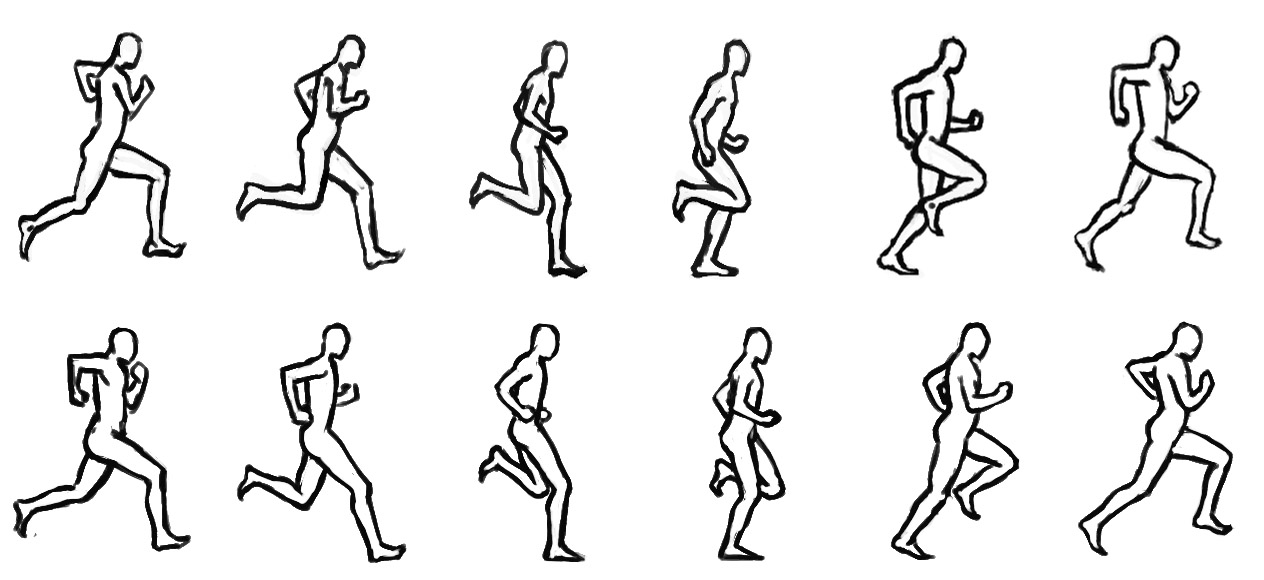
\includegraphics[width=9cm]{recursos/imagens/running.jpg}  \end{figure}


\lstinputlisting{recursos/codigos/clique.html}






\section{Referências Bibliográficas}

\noindent GEARY,David. \textbf{Core HTML5 Canvas: Graphics, Animation, and Game Development}. 2012.

\noindent https://www.tecmundo.com.br/navegador/2254-o-que-e-html-5-.htm

\noindent http://www.linhadecodigo.com.br/artigo/3488/entendendo-a-tag-canvas-no-html-5.aspx

\noindent https://pt.wikipedia.org/wiki/HTML5

\noindent https://developer.mozilla.org/pt-BR/docs/Web/HTML/HTML5

\noindent http://www.techtudo.com.br/artigos/noticia/2011/12/o-que-e-html5.html




\end{document}